\chapter{Teorema del campionamento} 

\begin{figure}[h]
    \centering
    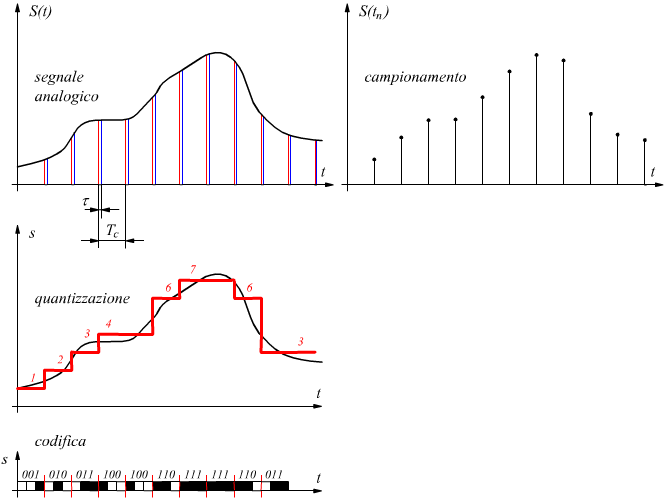
\includegraphics[scale = 0.6]{Campionamento segnale.png}
\end{figure}  

\newpage 

\section{Cosa è il campionamento e quali segnali soddisfano questo tipo di rappresentazione} 

Come la trasformata di Forurier, anche il teorema del campionamento può essere visto come una 
possibile rappresentazione del segnale. \newline 

Il campionamento non modifica il dominio del segnale s(t), quindi il dominio del segnale campionato 
rimane quello dei tempi. \newline 

I segnali che possono essere campionati sono quelli limitati in banda, con banda compresa (in pulsazione) tra 
$-2\pi B$ e $2\pi B$. \newline 

Se consideriamo B costante, appartengono alla classe i segnali che non vengono alterati nel transito 
attraverso un filtro passa-basso ideale con banda $2 \pi B$. \newline 

Un esempio grafico di un segnale campionabile: 

\begin{figure}[h]
    \centering
    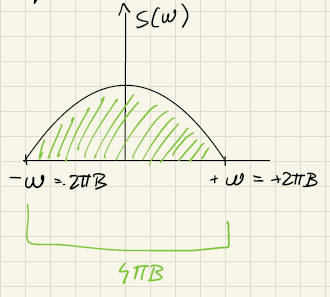
\includegraphics[scale = 0.6]{Segnale campionabile schema.PNG}
\end{figure}  

Il teorema del campionamento stabilisce che la conoscenza del segnale s(t) è del tutto 
equivalente alla conoscenza dei suoi campioni $s(k T_c)$, con k variabile intera, 
ottenuti calcolando s(t) per $t=kT_c$. \newline 

$T_c$ prende il nome di intervallo (o tempo) di campionamento. \newline 

Il suo inverso 
{
    \Large 
    \begin{equation}
        f_c = \frac{1}{T_c}    
    \end{equation}
}

è la frequenza di campionamento e rappresenta il numero di campioni del segnale per unità di tempo 
che è necessario considerare ai fini della rappresentazione. \newline 

Quindi, grazie a questo teorema, conoscere i campioni ogni $T_c$ è come conoscere tutto s(t) continuo. \newline 

Come ogni rappresentazione, non solo è necessaria la procedura per definire i campione dal segnale s(t), 
ma è anche necessaria la procedura inversa. \newline 

Consideriamo il segnale s(t) e la sua trasformata di Forurier $S(\omega)$. \newline 

Possiamo vedere $S(\omega)$ come alla rappresentazione elementare (all'interno di un periodo) di un segnale periodico in $\omega$ con periodo pari a $4\pi B$ 
in cui il segnale è centrato in $\omega = 0$. \newline 

Il segnale poi, viene periodicizzato nello spettro del segnale, proprietà molto importante nel campionamento. \newline 

In quanto periodica, la funzione così ottenuta può infatti essere sviluppata in serie di Fourier: 
rispetto alla notazione classica (in cui il segnale che viene sviluppato è una funzione del tempo) 
occorre sostituire t con $\omega$ e tener conto del fatto che il periodo vale $4 \pi B$. \newline 

{
    \Large 
    \begin{equation}
        S(\omega) 
        = 
        \frac{1}{\sqrt{4\pi B}} 
        \sum_{k = -\infty}^{+ \infty} 
        c_k e^{\frac{\jmath k \omega}{2B}}
    \end{equation}
}

{
    \Large 
    \begin{equation}
        c_k 
        = 
        \frac{1}{\sqrt{4 \pi B}} 
        \int_{-2 \pi B}^{2 \pi B}
        S(\omega) e^{-\frac{\jmath k \omega}{2B}} 
        d\omega
    \end{equation}
}

\newpage 

\subsection{Dimostrazione del Teorema del campionamnto}

Il segnale s(t) può essere espresso come anti-trasformata di $S(\omega)$, cioè: 

{
    \Large 
    \begin{equation}
        s(t) 
        = 
        \frac{1}{2 \pi} 
        \int_{-2\pi B}^{2\pi B} 
        S(\omega) e^{\jmath \omega t} 
        d\omega
    \end{equation}
}

Siccome il segnale s(t) è limitato in banda, risulta che: 

{
    \Large 
    \begin{equation}
        c_k 
        = 
        \sqrt{\frac{\pi}{B}}
        s(-\frac{k}{2B})
    \end{equation}
}

Sapendo che: 

{
    \Large 
    \begin{equation}
        T_c 
        = 
        \frac{1}{2B}
    \end{equation}
}

possiamo scrivere: 

{
    \Large 
    \begin{equation}
        c_k = \sqrt{\frac{\pi}{B}} s(-k T_c)
    \end{equation}
}

Questa ultima equazione esprime esplicitamente il teorema del campionamento. \newline 

Se infatti è vero che la conoscenza dei coeffiecienti $c_k$ è equivalente alla conoscenza della funzione 
$S(\omega)$ e quindi di s(t), questa ultima equazione ci dimostra che questi coefficienti possono essere determinati 
campionando il segnale s(t) in corrispondenza di multipli di $T_c$. \newline 

Un segnale limitato in banda non è necessariamente descritto dall'infinità non numerabili di valori 
che esso assume in ciascuno dei possibili istanti distinti nel tempo; 
per la sua completa conoscenza è sufficiente la determinazione dei valori che esso assume in corrispondenza di tutti e soli gli 
instanti multipli di $\frac{1}{2B}$. \newline 

\newpage 

\section{Ricostruzione del segnale s(t) partendo dai coefficienti} 

Partendo dalla definizione di segnale in $\omega$: 

{
    \Large 
    \begin{equation}
        S(\omega) 
        = 
        \frac{1}{\sqrt{4\pi B}} 
        \int_{k = -\infty}^{+ \infty} 
        c_k e^{\frac{\jmath k \omega}{2B}}
    \end{equation}
}

e sapendo che $c_k$, per un segnale limitato in banda, vale: 

{
    \Large 
    \begin{equation}
        c_k = \sqrt{\frac{\pi}{B}} s(-k T_c)
    \end{equation}
}

possiamo scrivere che $S(\omega)$ diventa: 

{
    \Large 
    \begin{equation}
        S(\omega) 
        = 
        \sum_{k = -\infty}^{+ \infty}
        \frac{1}{2B}
        s(-k T_c) e^{\jmath k \omega T_c}
    \end{equation}
}
Considerando solo l'intervallo di frequenze $[-2 \pi B, 2 \pi B]$ in cui è allocato il 
segnale s(t) e sostituendo -k con k, avremo che: 

{
    \Large 
    \begin{equation}
        S(\omega) 
        = 
        \sum_{k = -\infty}^{\infty} 
        \frac{1}{2B}
        s(kT_c) e^{-\jmath k \omega T_c}
        \text{ in } 
        -2\pi B \leq \omega \leq 2\pi B
    \end{equation}
}

Anti-trasformando $S(\omega)$, abbiamo che: 

{
    \Large 
    \begin{equation}
        \sum_{k = - \infty}^{+\infty} 
        s(kT_c) \frac{\sin[2\pi B(t-kT_c)]}{2 \pi B(t - kT_c)}
    \end{equation}
}

Siccome $\frac{\sin[2\pi B(t-kT_c)]}{2 \pi B(t - kT_c)}$, che prende il nome di funzione sinc, 
che ha massimo uguale a 1 in $t=kT_c$, prende il nome di funzione di campionamento. \newline 

Al variare di k, le funzione di campionamento che hanno la stessa struttura qualunque sia il segnale da rapppresentare, 
sono tra loro ortogonali. \newline 

Si hanno dunque condizioni analoghe a quelle dei segnali con sviluppo in serie di Forurier.\newline 

I campioni del segnale prendono dunque il posto dei coefficienti dello sviluppo in serie di Forurier. \newline 

\newpage 

\section{Dualità tempo-frequenza nel campionamento} 

Un'ulteriore considerazione riguardo il valore di $f_c$ è che, dalla definizione di $f_c$ e la relazione con B, abbiamo che: 

{
    \Large 
    \begin{equation}
        f_c = \frac{1}{T_c} = \frac{1}{\frac{1}{2B}} = 2B 
    \end{equation}
}

Quindi: 

{
    \Large 
    \begin{equation}
        f_c \geq 2B
    \end{equation}
}


All'aumentare di B, anche $f_c$ aumenta, tanto che al limite, per $B \rightarrow \infty$, 
il campionamento dovrebbe considerare tutti i possibili istanti temporali. \newline 

\newpage 

\section{Tipi di campionamento} 

In questa sezione analizzeremo quattro tipi di campionamento: 

\begin{itemize}
    \item Campionamento ideale 
    \item Campionamento naturale 
    \item Campionamento istantaneo 
    \item Campionamento di segnali passa-banda 
\end{itemize}

\newpage 

\subsection{Campionamento ideale}

Per campionamento ideale si intende il campionamento di un segnale utilizzando il 
famoso impulso matematico (Delta di Dirac), la quale ha durata infinitesima, ma ampiezza corrispondente infinita. \newline 

Consideriamo una successione di impulsi matematici: 

{
    \Large 
    \begin{equation}
        s_p 
        = 
        \sum_{k = -\infty}^{\infty} 
        \delta (t - k T_c)
    \end{equation}
}

Moltiplicando $s_p$ per s(t), possiamo svolgere un campionamento ideale. \newline 

Il segnale campionato in modo ideale sarà: 

{
    \Large 
    \begin{equation}
        \begin{split}
            s_c (t) 
            &= 
            s(t) \cdot s_p (t) 
            \\ 
            &= 
            s(t) \cdot \sum_{k = -\infty}^{\infty} \delta (t - k T_c)
            \\ 
            &= 
            \sum_{k = -\infty}^{\infty} s(k T_c) \delta (t - k T_c)
        \end{split} 
    \end{equation}
}

Avendo a che fare con una Delta di Dirac, nella realtà non riusciremo mai a realizzare un campionamento ideale. \newline 

Andando nel dominio in $\omega$, avremo che la successione di impulsi matematici $s_p (t)$ sarà: 

{
    \Large 
    \begin{equation}
        S_p (\omega) 
        = 
        \omega_c \sum_{k = - \infty}^{+ \infty} \delta (\omega - k \omega_c)    
    \end{equation}
}

in cui: 

{
    \Large 
    \begin{equation}
        \omega_c = 2\pi f_c = \frac{2\pi}{T_c}
    \end{equation}
}

Quindi, la trasformata di Fourier della sequenza di impulsi matematici distanziati nel tempo di $T_c$ è dunque, 
a sua volta, una sequenza di impulsi matematici distanziati in pulsazione di $\omega_c$. \newline 

Ricordando la proprietà della delta di Dirac, in cui la convoluzione con una funzione generica restituisce la funzione stessa centrata 
dove era posizionata la delta di Dirac, si può concludere che: 

{
    \Large 
    \begin{equation}
        \begin{split}
            S_c (\omega) 
            &= 
            \frac{\omega_c}{2 \pi} 
            \sum_{k = - \infty}^{ + \infty} 
            S(\omega - k \omega_c) 
            \\ 
            &= 
            \frac{1}{T_c} 
            \sum_{k = - \infty}^{ + \infty} 
            S(\omega - k \omega_c) 
        \end{split}
    \end{equation}
} 

Questi schemi possono essere utili per visualizzare le equazioni: 

\begin{figure}[h]
    \centering
    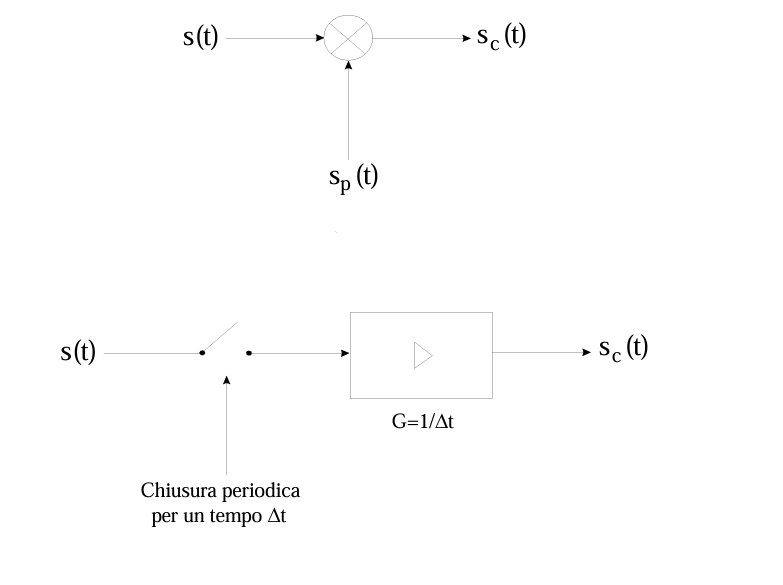
\includegraphics[scale = 0.6]{Campionamento ideale.PNG}
\end{figure}  

\newpage 

Ora facciamo lo step inverso. \newline 

Partendo dai campioni, possiamo riottenere il segnale: per fare ciò, ci serve un filtro passa-basso. \newline 

Lo schema generale del sistema diventa: 

\begin{figure}[h]
    \centering
    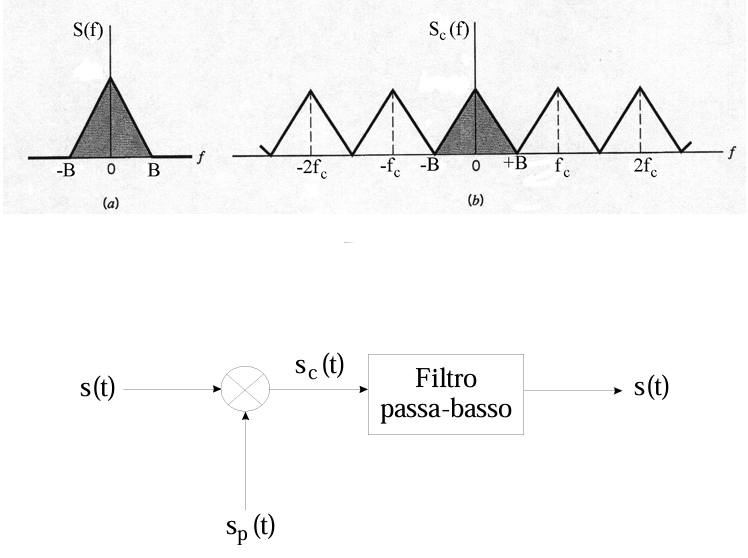
\includegraphics[scale = 0.6]{Dai campioni ideali al segnale.PNG}
\end{figure}  



Ponendo: 

{
    \Large 
    \begin{equation}
        f_c = 2B
    \end{equation}
} 

ci permette di non modificare il segnale originale senza avere distorsione. \newline 

Se invece: 

{
    \Large 
    \begin{equation}
        f_c < 2B
    \end{equation}
}

si sta svolgendo un sottocampionamento (undersampling in inglese). \newline 

Sottocampionando il segnale, questo ultimo avrà delle distorsioni, quindi degli effetti non lineari. \newline 

Un esempio di un sottocampionamento: 

\begin{figure}[h]
    \centering
    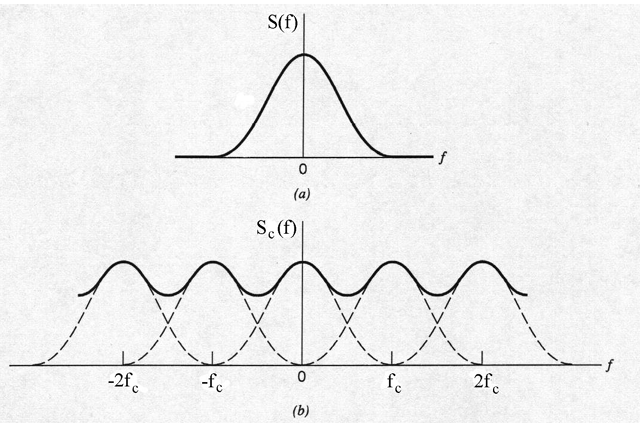
\includegraphics[scale = 0.6]{Esempio di sotto-campionamento.PNG}
\end{figure}  

\newpage 

Se invece si sovra-campiona, quindi: 

{
    \Large 
    \begin{equation}
        f_c > 2B
    \end{equation}
}

si sta sovracampionando (in inglese oversampling) il segnale. \newline 

L'assunzione di una frequenza di campionamento $f_c$ maggiore di quella strettamente necessaria, 
non altera le prestazioni del campionamento, anzi, ne semplifica l'implementazione pratica. \newline 

La condizione: 

{
    \Large 
    \begin{equation}
        f_c \geq 2B
    \end{equation}
} 

prende il nome di condizione di Nyquist. \newline 

Un esempio di sovra-campionamento: 

\begin{figure}[h]
    \centering
    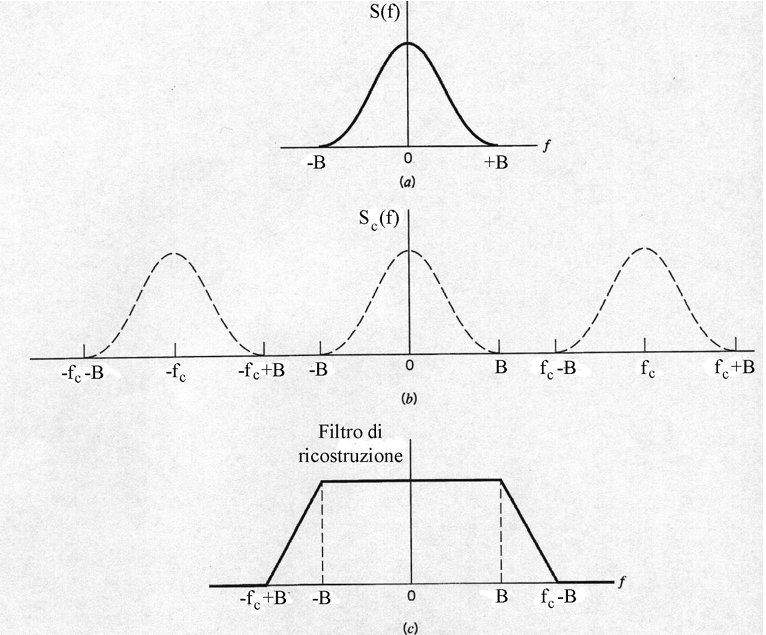
\includegraphics[scale = 0.6]{Esempio di segnale sovracampionato.PNG}
\end{figure}  

\newpage 

\subsection{Campionamento naturale} 

L'idealità dello schema di campionamento ideale sta nella impossibilità di utilizzare 
come funzione campionante una successione di Delta di Dirac. \newline 

Considerando questo sistema: 

\begin{figure}[h]
    \centering
    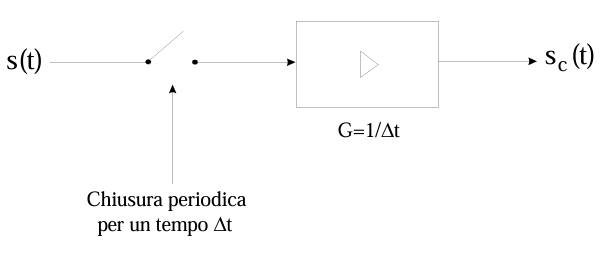
\includegraphics[scale = 0.6]{Campionamento naturale.PNG}
\end{figure}  

e $\Delta t$ un tempo infinitesimo, allora non avremo più una successione di impulsi, bensì 
una successione di impulsi rettangolari con seguente funzione: 

{
    \Large 
    \begin{equation}
        s_p (t) 
        = 
        \sum_{k= -\infty}^{+\infty}
        s_l (t- k T_c)
    \end{equation}
}

in cui $s_l (t)$ è l'impulso rettangolare unitario: 

{
    \Large 
    \begin{equation}
        s_l (t) 
        = 
        \begin{cases}
            1 \text{ se } \abs{t} \leq \frac{\Delta t}{2} \\ 
            0 \text{ se } \abs{t} > \frac{\Delta t}{2} 
        \end{cases}
    \end{equation}
}

Quando il segnale $s_p (t)$ è moltiplicao per s(t), il segnale campionato segue esattamente l'andamento del segnale in ingresso, 
ma limitatamente agli intervalli, periodici, di durata $\Delta t$. \newline 

Dal punto di vista grafico, il campionamento naturale di un segnale sarà: 

\begin{figure}[h]
    \centering
    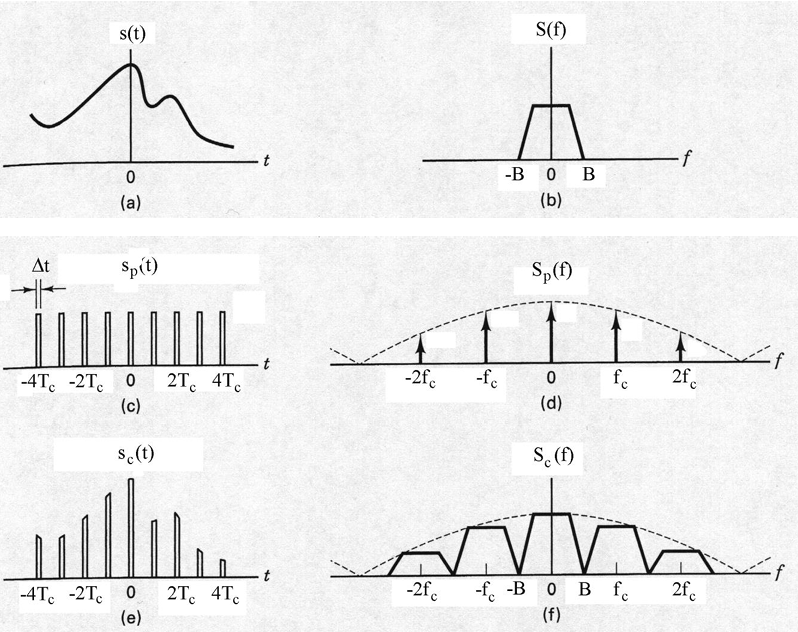
\includegraphics[scale = 0.7]{Segnale con campionamento naturale.PNG}
\end{figure}  

Più che una conoscenza puntuale del segnale s(t), si può qui parlare di conoscenza "intervallata" in porzioni di tempo 
significativamente più piccole del dominio originale. \newline 

Rispetto al caso ideale, si ha una ridondanza di informazione. \newline 

L'espressione matematica del segnale campionato, è, in questo caso, data da: 

{
    \Large 
    \begin{equation}
        \begin{split}
            s_c (t)
            &= 
            s(t) \cdot s_p (t)
            \\ 
            &= s(t) \sum_{k = -\infty}^{+ \infty} s_l (t - kT_c) 
        \end{split}
    \end{equation}
}

Il segnale campionante $s_p (t)$ è periodico, e dunque la sua trasformata vale: 

{
    \Large 
    \begin{equation}
        \begin{split}
            S_p (\omega) 
            &= 
            \omega_c 
            \sum_{k = -\infty}^{+ \infty}
            S_l (\omega) \delta (\omega - k \omega_c)
            \\ 
            &= 
            \omega_c 
            \sum_{k = -\infty}^{+ \infty}
            \Delta t 
            \frac{\sin(\omega \frac{\Delta t}{2})}{\omega \frac{\Delta t}{2}} 
            \delta (\omega - k \omega_c) 
            \\ 
            &= 
            \omega_c 
            \sum_{k = -\infty}^{+ \infty}
            \Delta t 
            \frac{\sin(k \omega_c \frac{\Delta t}{2})}{k \omega_c \frac{\Delta t}{2}} 
            \delta (\omega - k \omega_c)
        \end{split}
    \end{equation}
}

Considerando $S_l (\omega)$ la trasformata di Fourier dell'impulso rettangolare, il segnale campionato sarà del tipo: 

{
    \Large 
    \begin{equation}
        S_c (\omega) 
        = 
        \frac{\Delta t}{T_c} 
        \sum_{k = -\infty}^{+ \infty} 
        \frac{\sin (k \omega_c \frac{\Delta t}{2})}{k \omega_c \frac{\Delta t}{2}} 
        S(\omega - k \omega_c)
    \end{equation}
}

A meno del fattore $\Delta t$ e il conributo per $k = 0$, 
le due repliche sono moltiplicate per $\frac{\sin (k \omega_c \frac{\Delta t}{2})}{k \omega_c \frac{\Delta t}{2}} < 1$, 
ma mantengono esattamente la forma dello spettro originale, e dunque non sono distorte. \newline 

\newpage 

\subsection{Campionamento istantaneo}

Un primo, ma importante, passo verso la numerizzazione del segnale si ottiene considerando il campionamento istantaneo. \newline 

Un esempio di campionamento istantaneo: 

\begin{figure}[h]
    \centering
    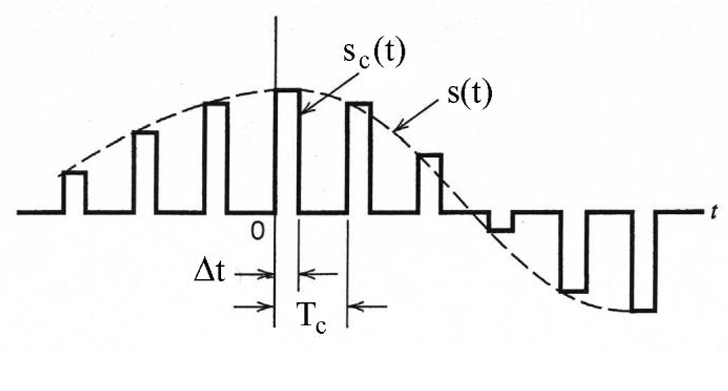
\includegraphics[scale = 0.6]{Esempio di segnale con campionamento istantaneo.PNG}
\end{figure}  

Rispetto al campionamento naturale, all'interno degli intervalli di durata $\Delta t$, 
il segnale campionato non segue il segnale originale, ma conserva il valore negli istanti di campionamento. \newline 

Quindi, il segnale con campionamento istantaneo è un segnale distorto, in altre parole, il segnale 
campionato in modo istantaneo è diverso da quello originale. \newline 

In pratica, il valore campionarto nell'istante $t = kT_c$ viene prolungato per l'intero intervallo $kT_c \leq t \leq kT_c + \Delta t$. \newline 

Un esempio di circuito per un campionamento istantaneo è quello del sample and hold (in italiano campionamento e tenuta). 

\begin{figure}[h]
    \centering
    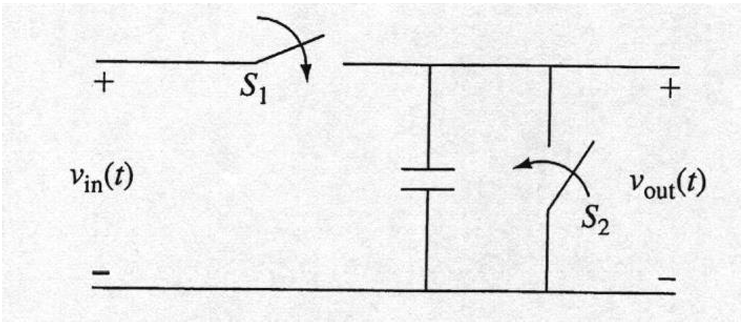
\includegraphics[scale = 0.6]{Circuito Sample and hold.PNG}
\end{figure} 

Il fatto che negli intervalli di durata $\Delta t$ il segnale campionato non segua l'andamento di s(t) ma venga forzato a rimanere costante, introduce evidentemente 
un'alternazione che è ragionevole pensare possa tradursi in una distorsione del segnale ricostruito. \newline 

Per valutare l'entità di questa distorsione, scriviamo l'entità di questa distorsione, scriviamo l'espressione del segnale campionato nel cao di campionamento istantaneo: 

{
    \Large 
    \begin{equation}
        s_c (t) 
        = 
        \sum_{k = - \infty}^{\infty}
        s(kT_c) 
        s_l (t-kT_c)
    \end{equation}
} 

Utilizzando la proprietà della convoluzione, $s_c (t)$ possiamo riscriverla come: 

{
    \Large 
    \begin{equation}
        s_c (t) = s_l \otimes s(t) \sum_{k = -\infty}^{\infty} \delta (t - k T_c)
    \end{equation}
}

dove: 

{
    \Large 
    \begin{equation}
        s_l (t) \otimes \delta(t - kT_c) = s_l (t - kT_c)
    \end{equation}
}

Applicando la proprietà della convoluzione e quella del prodotto, la trasformata di Fourier 
di $s_c (t)$ potrà riscriversi come: 

{
    \Large 
    \begin{equation}
        \begin{split}
            S_c (\omega) 
            &=
            \frac{1}{T_c} S_l (\omega) 
            \sum_{k = - \infty}^{\infty} 
            S(\omega -k \omega_c) 
            \\ 
            &=
            \frac{\Delta t}{T_c} 
            \frac{\sin(\omega \frac{\Delta t}{2})}{\omega \frac{\Delta t}{2}} 
            \sum_{k = -\infty}^{\infty} 
            S(\omega - k\omega_c)
        \end{split}
    \end{equation}
}

Confronta i tre casi di campionamento in $\omega$: \newline 

\textbf{Campionamento istantaneo}

{
    \Large 
    \begin{equation}
        S_c (\omega) = 
        \frac{\Delta t}{T_c} 
        \frac{\sin(\omega \frac{\Delta t}{2})}{\omega \frac{\Delta t}{2}} 
        \sum_{k = -\infty}^{\infty} 
        S(\omega - k\omega_c)
    \end{equation}
}

\textbf{Campionamento natuale}

{
    \Large 
    \begin{equation}
        S_c (\omega) = 
        \frac{\Delta t}{T_c} 
        \frac{\sin(\omega \frac{\Delta t}{2})}{k \omega_c \frac{\Delta t}{2}} 
        \sum_{k = -\infty}^{\infty} 
        S(\omega - k\omega_c)
    \end{equation}
}

\textbf{Campionamento ideale} 

{
    \Large 
    \begin{equation}
        S_c (\omega) = 
        \frac{1}{T_c} 
        \sum_{k = -\infty}^{\infty}
        S(\omega - k\omega_c)
    \end{equation}
}

notiamo che le singole repliche dello spettro del segnale originale sono, 
in questo caso, moltiplicate non per un valore costante (come avviene nel caso di campionamento naturale) 
ma, nel campionamento instantaneo, lo spettro segnale viene moltiplicato per una funzione in $\omega$. \newline 

In particolare, il filtro passa-basso di ricostruzione che isola la replica centrata nell'origine, 
darà in uscita un segnale $s^{'} (t)$ il cui spettro vale: 

{
    \Large 
    \begin{equation}
        S^{'} (\omega) = 
        \frac{\Delta t}{T_c} 
        \frac{\sin(\omega \frac{\Delta t}{2})}{\omega \frac{\Delta t}{2}} 
        S(\omega)
    \end{equation}
}

Si tratta dunque dello spettro di $S(\omega)$ moltiplicato per la funzione $sinc(\omega \frac{\Delta t}{2})$. 

Quindi, per riassumere, contrariamente agli altri tipi di campionamento, si avrà che: 

{
    \Large 
    \begin{equation}
        s^{'} (t) \neq s(t)
    \end{equation}
}

Un esempio dello spettro tra il campionamento ideale e campionamento istantaneo: 

\begin{figure}[h]
    \centering
    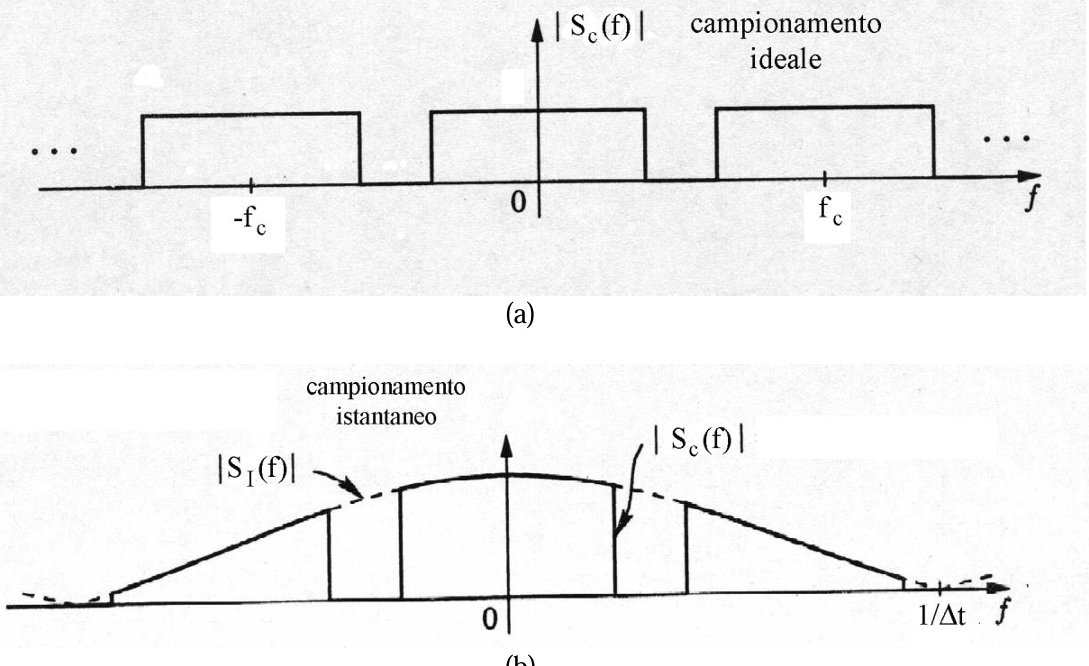
\includegraphics[scale = 0.6]{Differenze tra campionamento ideale e campionamento istantaneo.PNG}
\end{figure} 

\newpage 

Da questo confronto, possiamo svolgere due considerazioni. \newline

La prima considerazione da svolgere è che l'entità della distorsione è legata al valore di $\Delta t$. \newline 

Consideriamo il rapporto tra $\abs{S^{'} (\omega)}$ e $\abs{S(\omega)}$: 

{
    \Large 
    \begin{equation}
        \abs{\frac{S^{'} (\omega)}{S(\omega)}}
        = 
        \frac{\Delta t}{T_c}
        \abs{\frac{\sin(\omega \frac{\Delta t}{2})}{\omega \frac{\Delta t}{2}}} 
    \end{equation}
}

Di conseguenza, in $\omega = 0$: 

{
    \Large 
    \begin{equation}
        \left|\frac{S^{'} (\omega)}{S(\omega)} \right|_{\omega = 0} 
        = 
        \frac{\Delta t}{T_c}
    \end{equation}
} 

e 

{
    \Large 
    \begin{equation}
        \begin{split}
            \left|\frac{S^{'} (\omega)}{S(\omega)} \right|_{\omega = 2 \pi B} 
            &= 
            \frac{\Delta t}{T_c} 
            \abs{\frac{\sin(\pi B \Delta t)}{\pi B \Delta t}} 
            \\ 
            &= 
            \frac{2}{\pi} 
            \sin(\frac{\pi}{2} \frac{\Delta t}{T_c})
        \end{split}        
    \end{equation}

}

dove: 

{
    \Large 
    \begin{equation}
        B = \frac{1}{2 T_c} 
    \end{equation}
}

e 

{
    \Large 
    \begin{equation}
        \frac{\Delta t}{T_c} < 1        
    \end{equation}
}

Se consideriamo il rapporto tra i due rapporti di $S^{'}(\omega)$ e $S(\omega)$: 

{
    \Large 
    \begin{equation}
        \frac{\left|\frac{S^{'} (\omega)}{S(\omega)} \right|_{\omega = 2 \pi B}}{\left|\frac{S^{'} (\omega)}{S(\omega)} \right|_{\omega = 0}} 
        = 
        \frac{\sin(\frac{\pi}{2} \frac{\Delta t}{T_c})}{\frac{\pi}{2} \frac{\Delta t}{T_c}}
    \end{equation}
}

Se: 

{
    \Large 
    \begin{equation}
        \frac{\left|\frac{S^{'} (\omega)}{S(\omega)} \right|_{\omega = 2 \pi B}}{\left|\frac{S^{'} (\omega)}{S(\omega)} \right|_{\omega = 0}} 
        = 
        1  
    \end{equation}
}

la distorsione sarebbe nulla all'interno della banda del segnale. \newline 

Quanto minore è il rapporto $\frac{\Delta t}{T_c}$, tanto minore risulta la distorsione (si parla di effetto finestra). \newline 

Per alcune applicazioni un valore di $\frac{\Delta t}{T_c} < 0.1$ è già sufficiente per garantire distorsione trascurabile. \newline 


Un'altra considerazione tra campionamento ideale e campionamento instantaneo è la distorsione introdotta dall'effetto finestra, la quale è equalizzabile. \newline 

Visto che si conosce l'andamento in frequenza della funzione distorcente, è sufficente incorporare 
nell'aparato di ricostruzione un filtro con funzione di trasferimento: 

{
    \Large 
    \begin{equation}
        H_{eq} (\omega) = 
        \frac{A e^{\jmath \omega t_d}}{S_l (\omega)} 
    \end{equation}
}

perchè la distorsione venga eliminata e si riottenga il segnale ricostruito come nel campionamento naturale. \newline 

Il termine $e^{\jmath \omega t_d}$ è necessario per tener conto del ritardo necessariamente introdotto dall'equalizzazione reale; 
A è un coefficiente moltiplicativo. \newline 

\newpage 

\subsection{Campionamento di segnali passa-banda} 

Si consideri il segnale la cui trasformata di Fourier è la seguente: 

\begin{figure}[h]
    \centering
    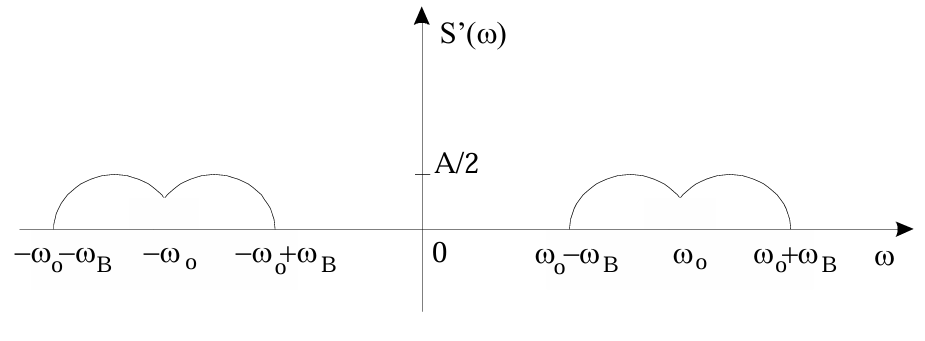
\includegraphics[scale = 0.6]{Esempio di segnale trasformato in Fourier.PNG}
\end{figure}

Si può campionare ad una frequenza minore della condizione di Nyquist grazie ai buchi nelle bande di frequenza. \newline 

\newpage 

\section{Codifica PCM e sua applicazione a segnali di interesse pratico} 

Lo schema a blocchi di un sistema che utilizza la modulazione impulsiva codificata (PCM: Pulse Code Modulation): 

\begin{figure}[h]
    \centering
    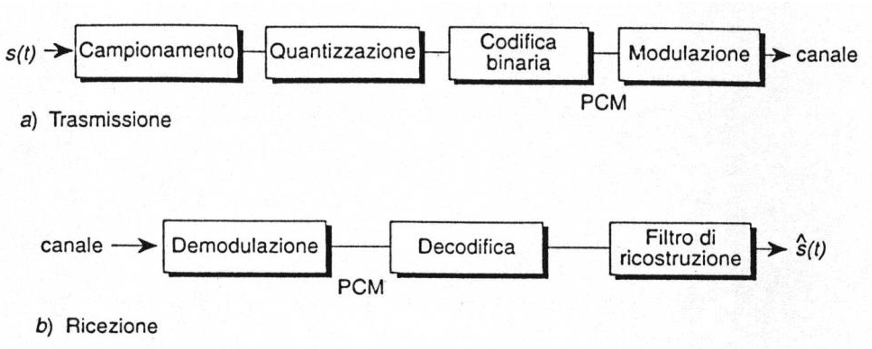
\includegraphics[scale = 0.6]{PCM Schema a blocchi.PNG}
\end{figure}

Il punto di partenza è costituito da un segnale analogico s(t) di banda limitata, 
che viene campionato, in accordo con il teorema di campionamento,con una frequenza almeno pari a 2B. \newline 

In tal modo, il segnale variabile in modo continuo nel tempo viene trasformato in una seguenza, discreta, di campioni. \newline 

Le ampiezze dei campioni, peraltro, possono essere qualisiasi (compatibilmente con la dinamica del segnale s(t)). \newline 

Per ricavare la frequenza di cifra del segnale PCM, è sufficiente guardare alle operazioni che conducono dal segnale analogico s(t) al segnale numerico PCM: 

\begin{itemize}
    \item il campionamento comporta che venga prelevato un campione ogni $T_o = \frac{1}{f_o} \leq \frac{1}{2B} [s]$ (la frequenza di campionamento è stata qui indicata con $f_o$)
    \item il tenpo riservato alla trasmissione di un simbolo M-ario non può eccedere $\frac{1}{2B}$: si assume, di solito, il valore massimo 
    \item sostituendo una sequenza binaria al generico simbolo M-ario, ciascuna cifra binaria avrà durata massima pari a $\frac{1}{2B \cdot \log_2 M}$ in quanto il tempo riservato alla trasmissione di un simbolo M-ario deve ora essere ripartito tra i $\log_2 M$ simboli binari
\end{itemize}


La frequenza di cifra del PCM sarà: 

{
    \Large 
    \begin{equation}
        F_c = 2B \cdot \log_2 M
    \end{equation}
}

Per i segnali di interesse pratico, i valori di B e di M sono stardatizzati. \newline 

\newpage 
.
\newpage
.
\newpage
